% --- page 25 ---
% CONTINUES: the AKS discussion ends (p.24) with the remark that RSA needs factorization.

\section{Factorization Algorithms}
% ============================================================

John Pollard gave two algorithms for this problem. Both are developed below: the $\rho$-method, and the $p-1$ method.

\subsection{A birthday count}

\begin{quote}
How many people must we gather so that the probability that two of them share a birthday is at least $1/2$?
\end{quote}

Assuming $365$ equally likely days and ignoring leap years, the probability that $k$ people all have distinct birthdays is
\[
    \frac{365}{365}\cdot\frac{364}{365}\cdot\frac{363}{365}\cdots\frac{365-k+1}{365}
    = \prod_{i=0}^{k-1}\frac{365-i}{365}.
\]
The largest $k$ for which this product is still greater than $1/2$ is $k=22$. Thus, with $23$ people, the probability of at least one shared birthday is greater than $1/2$.

For scale,
\[
    \sqrt{365}\approx 19, \qquad \sqrt{2\cdot 365}\approx 27,
\]
and $23$ lies between these two estimates.
% The approximation $\lceil\sqrt{2m\log 2}\rceil$ below matches $23$ when $\log$ is natural: $\sqrt{2\ln 2}\approx 1.177$ and $1.177\sqrt{365}\approx 22.5$.

The same counting is what a factor search costs. Suppose $m$ is an unknown factor of $n$, and $x_1,x_2,x_3,\ldots$ are random integers. A collision of residues,
\[
    x_1\equiv x_2\pmod{m},
\]
is exactly the condition $m\mid(x_1-x_2)$.
% FIX p.25: the mark between $x_1$ and $x_2$ is only a short stroke; it is read as a minus, since the line is the definition of the congruence just above it.
One expects the residue classes modulo $m$ to be equally likely. The question is then the birthday problem with only $m$ possible birthdays.

% --- page 26 ---

How many people must we gather so that the probability that two of them share a birthday is at least $1/2$? The answer is about
\[
    \bigl\lceil\sqrt{2m\log 2}\bigr\rceil
\]
people. More generally, for the probability to be $1-\varepsilon$ for any fixed $\varepsilon>0$, the number of people required is still $O(\sqrt{m})$.

\subsection{Pollard's \texorpdfstring{$\rho$}{rho}-method}

If the unknown modulus is an integer $m$, then $O(\sqrt{m})$ random integers are enough to find two that are congruent modulo $m$, almost certainly.

\paragraph{Method.}
\begin{itemize}[leftmargin=1.4em]
    \item Choose a polynomial $f(x)\in\Z[x]$ of degree at least $2$. The running choice is $f(x)=x^2+1$.
    \item Let $x_0=2$, and define $x_{i+1}=f(x_i)$. In practice the terms are reduced modulo $n$.
    \item Look at the differences $x_i-x_j$ modulo $n$, until an index $k$ is found for which
    \[
        x_k\not\equiv x_j\pmod{n}
        \qquad\text{for all }1\le j<k,
    \]
    but $\gcdop(x_k-x_j,n)\ne 1$ for some $j<k$.
    % UNCLEAR p.26: the bullet opens with words that read as ``look for at $(x_i-x_j)$ modulo $n$''.
    % FIX p.26: the scan writes $1\le j\le k$. The case $j=k$ is empty, so the range is $j<k$.
    \item It is more likely than not that a factor of $n$ appears within $O(n^{1/4})$ steps.
\end{itemize}

The exponent $1/4$ is the birthday count on a prime factor. If $m\mid n$ and the residues modulo $m$ behave randomly, about $\sqrt{m}$ terms produce a collision modulo $m$. In the balanced case $m\le\sqrt{n}$, so $\sqrt{m}\le n^{1/4}$.

% --- page 27 ---

\begin{example}[A $\rho$-iteration]
Take $n=37351$ and $f(x)=x^2+1$, starting at $x_0=2$. The first terms need no reduction:
\[
    x_1=5, \qquad x_2=26, \qquad x_3=677.
\]
Then $x_3^2+1=458330$, and $458330-12\cdot 37351=10118$, so
\begin{align*}
    x_4 &\equiv 10118,\\
    x_5 &\equiv 32185,\\
    x_6 &\equiv 18943,\\
    x_7 &\equiv 6193 \pmod{37351}.
\end{align*}
Hence $x_7-x_0=6191$ and
\[
    \gcdop(6191,37351)=41.
\]
Since $37351=41\cdot 911$, the gcd is a prime factor of $n$.
\end{example}

\begin{remark}
% FIX p.27: the scan writes $x_4\equiv 3146$, $x_5\equiv 36653$, $x_6\equiv 1642$, then $x_6-x_0\equiv 1640$ and $\gcdop(1640,37351)=41$, with a crossed-out factorisation of $1640$ beside it (the second factor reads like ``$41.10$''; $1640=41\cdot 40$).
The scan continues from $x_4\equiv 3146$, which is not $677^2+1\bmod 37351$, and gets $x_5\equiv 36653$, $x_6\equiv 1642$, hence the same factor $41$ one step earlier.
\end{remark}

The graph is a tail into a cycle, the shape of the letter $\rho$. Given a composite $n$, a factor can certainly be found in $O(\sqrt{n})$ steps by testing divisors up to $\sqrt{n}$. The $O(n^{1/4})$ bound is only a likely cost.

\begin{figure}[H]
\centering
\begin{tikzpicture}[x=0.95cm,y=0.95cm,>=stealth,line cap=round]
    \node (x0) at (0,0) {$x_0$};
    \node (x1) at (1.45,0.52) {$x_1$};
    \node (x2) at (2.75,0.98) {$x_2$};
    \draw[->] (x0) -- (x1);
    \draw[->] (x1) -- (x2);
    % circle centre (5.55,2.55), radius 1.02; E is the entry, P the vertex before it
    \draw[dashed] (5.55,2.55) circle[radius=1.02];
    \coordinate (E) at (4.62,2.15);
    \coordinate (P) at (4.86,1.78);
    \draw[densely dotted] (3.05,1.12) -- (4.28,1.70);
    \draw[->] (4.28,1.70) -- (E);
    \node[anchor=south east] (labT) at (4.35,2.45) {$x_T=x_{T+M}$};
    \draw[->] (labT.south east) -- (E);
    \node[anchor=north] (labP) at (4.55,0.95) {$x_{T+M-1}$};
    \draw[->] (labP.north) -- (P);
    \node[anchor=west, align=left] at (6.75,1.85) {$\rho$-shape,\\ hence $\rho$-method.};
\end{tikzpicture}
\caption{Tail $x_0,x_1,x_2,\ldots$ entering the cycle at $x_T=x_{T+M}$. The dashed loop is the cycle; $x_{T+M-1}$ is the vertex just before the repeat.}
\end{figure}

\lectureheading{Lecture 17 (13/10/26)}

\paragraph{Pollard's $\rho$-algorithm, restated.}
If there are $n$ possible birthdays, all equally likely, then about
\[
    \bigl\lceil\sqrt{2n\log 2}\bigr\rceil
\]
people are needed before the probability that at least two share a birthday exceeds $1/2$.

The notes then indicate a general threshold. For any $\varepsilon>0$ one asks for a probability larger than $1/(1+\varepsilon)$. The number of samples that produces this probability is
\begin{equation}
    \sqrt{2n\log\frac{1+\varepsilon}{\varepsilon}} \;=\; O(\sqrt{n}).
    \label{eq:birthday-eps}
\end{equation}
% FIX p.27: the page writes $\sqrt{2n\log(*\varepsilon)}$, with the argument of the logarithm illegible, under the threshold $1/(1+\varepsilon)$. The collision probability is about $1-e^{-k^{2}/(2n)}$, which exceeds $1/(1+\varepsilon)$ once $k>\sqrt{2n\log((1+\varepsilon)/\varepsilon)}$. The target $1-\varepsilon$ on the previous page would put $\log(1/\varepsilon)$ under the square root instead. For fixed $\varepsilon>0$ either expression is $O(\sqrt{n})$.

% --- page 28 ---

\begin{example}[The iteration becomes periodic]
Take the same polynomial modulo $n=29$, again with $x_0=2$. Reducing $x^2+1$ at each step, and keeping the unreduced square when the notes do, gives
\begin{align*}
    x_0 &= 2,\\
    x_1 &= 5,\\
    x_2 &= 26,\\
    x_3 &= 677 \equiv 10,\\
    x_4 &\equiv 101 \equiv 14,\\
    x_5 &\equiv 197 \equiv 23 \equiv -6,\\
    x_6 &\equiv 37 \equiv 8,\\
    x_7 &\equiv 65 \equiv 7,\\
    x_8 &\equiv 50 \equiv 21 \equiv -8 \pmod{29}.
\end{align*}
One further step returns to $x_7$: using the representative $-8$,
\[
    x_9 \equiv (-8)^2+1 = 65 \equiv 7 \equiv x_7 \pmod{29}.
\]
So from $x_7$ onwards the sequence has period $2$.
\end{example}

\begin{figure}[H]
\centering
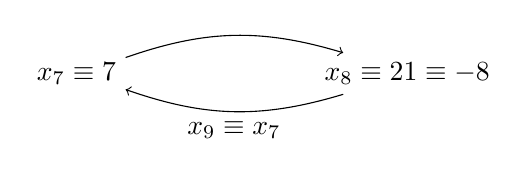
\begin{tikzpicture}
    \node (a) at (0,0) {$x_7\equiv 7$};
    \node (b) at (4.2,0) {$x_8\equiv 21\equiv -8$};
    \draw[->] (a) to[bend left=18] (b);
    \draw[->] (b) to[bend left=18] node[below] {$x_9\equiv x_7$} (a);
\end{tikzpicture}
\caption{The cycle found modulo $29$: the arrow in the notes identifies $x_9$ with $x_7$.}
\end{figure}

\begin{remark}
With $f(x)=x^2+1$, every term $x_i$ has to be stored before a useful divisor can be read off from a difference. (The formula $f(x)=x^2+1$ is struck through in the notes at this point.) The repair below tests only one difference per step.
\end{remark}

\paragraph{Repair.}
Replace the polynomial by $f(x)=x^2+c$ for a fixed integer $c$, and run two copies of the iteration from the same seed $x_0=y_0$:
\[
    x_{i+1}=f(x_i), \qquad y_{i+1}=f(f(y_i)).
\]
The fast copy is just the even terms of the slow copy, $y_i=x_{2i}$. At each step compute
\[
    \gcdop\bigl(|x_i-y_i|,\, N\bigr).
\]
If the gcd equals $1$, continue. If it equals $N$, change $f$ (a different $c$, or a different seed). If $1<\gcdop(|x_i-y_i|,N)<N$, the gcd is a factor of $N$.

\paragraph{Why the repair works.}
The sequence $(x_i)$, reduced modulo a factor $k$ of $N$, takes values in a finite set, so it is eventually periodic modulo $k$. There exist integers $T\ge 0$ and $M\ge 1$ such that
\begin{equation}
    x_{r+M}\equiv x_r\pmod{k}
    \qquad\text{for every }r\ge T.
    \label{eq:period}
\end{equation}

% --- page 29 ---

Now suppose $j>i$ and $x_j\equiv x_i\pmod{k}$. Then the indices have already passed the tail, so $i\ge T$, and they differ by a multiple of the period, $j\equiv i\pmod{M}$.

In particular,
\[
    x_{2i}\equiv x_i\pmod{k}
\]
as soon as $i\ge T$ and $2i\equiv i\pmod{M}$, that is $i\equiv 0\pmod{M}$. Among the $M$ consecutive integers
\[
    T,\; T+1,\; \ldots,\; T+M-1
\]
there is a multiple of $M$. That multiple is an admissible index (or the next multiple of $M$ is, which is at most $T+M$). For the corresponding $i$ one has $y_i=x_{2i}\equiv x_i\pmod{k}$, so $k$ divides $x_i-y_i$. Unless the same difference vanishes modulo $N$, the gcd with $N$ is a nontrivial factor.

\begin{theorem}
Let $S$ be a finite set with $m$ elements, let $f\colon S\to S$ be a map, and let $x_0\in S$. Write $x_i=f^{i}(x_0)$. Suppose there exist integers $T$ and $M$ such that
\[
    x_{r+M}=x_r \qquad\text{for every }r\ge T.
\]
Then $x_{2i}=x_i$ for some index $i$ with $1\le i\le T+M$.
\end{theorem}

\begin{remark}
% FIX p.29: the notes say ``if $f$ is sufficient'', which is read as ``sufficiently random''.
If $f$ is sufficiently random, then for large $m$ the expected value of the sum $T+M$ is about $1.253\sqrt{m}$. (The constant is $\sqrt{\pi/2}\approx 1.2533$, the expected length of the tail plus the cycle for a random function on a set of size $m$.)
\end{remark}

\subsection{Pollard's \texorpdfstring{$p-1$}{p-1} method}

This is the second of Pollard's algorithms. It is also the reason one has to be careful when choosing the secret primes in RSA.

Let $N=pq$ with $p$ and $q$ prime. If $p-1$ or $q-1$ factors into small primes, then $p$ and $q$ can be recovered from $N$.

Suppose there is an integer $L$ such that $(p-1)\mid L$ but $(q-1)\nmid L$. Write
\[
    L=(p-1)\,i
    = (q-1)\,j + k,
    \qquad 0<k<q-1.
\]

% --- page 30 ---

Take an integer $a$ with $\gcdop(a,N)=1$. Then $\gcdop(a,p)=\gcdop(a,q)=1$, and Fermat's theorem gives
\[
    a^{L}=(a^{p-1})^{i}\equiv 1\pmod{p},
\]
so $p$ divides $a^{L}-1$. On the other side,
\[
    a^{L}=a^{(q-1)j+k}=(a^{q-1})^{j}\,a^{k}\equiv a^{k}\pmod{q}.
\]
Hope that $a^{k}\not\equiv 1\pmod{q}$. Then $a^{L}\not\equiv 1\pmod{q}$, so $q$ does not divide $a^{L}-1$. Therefore
\[
    \gcdop(a^{L}-1,\, N)=p.
\]

\paragraph{How to choose $a$.}
The group $\units{q}$ has $\varphi(\varphi(q))$ primitive roots. For $q$ prime one has $\varphi(q)=q-1$, so this count is $\varphi(q-1)$. If $a$ is a primitive root modulo $q$, then $a^{k}\not\equiv 1\pmod{q}$ whenever $0<k<q-1$, and the hope above holds. The value $\varphi(q-1)$ is large when $q-1$ has no small prime factors, so in that case a random $a$ is reasonably likely to work. The running time is large when $p-1$ has a large prime factor, which is what one wants of an RSA prime.
% FIX p.30: the two facts are separate. A large $\varphi(q-1)$ makes a random base likely to satisfy $a^k\not\equiv 1\pmod q$. The cost is the size of the largest prime factor of $p-1$, not that count.

\paragraph{How to choose $L$.}
Suppose $p-1$ has only small prime factors. Then $(p-1)\mid n!$ for some $n$ that is still small, and
\[
    L=n!
\]
is a possible choice. One therefore tries to compute $\gcdop(a^{n!}-1,\, N)$, as follows.
\begin{itemize}[leftmargin=1.4em]
    \item Start with $a=2$.
    \item If the gcd equals $1$, increase $n$.
    \item If the gcd equals $N$, change $a$.
    \item If $1<\gcdop(a^{n!}-1,N)<N$, the gcd is a factor of $N$.
\end{itemize}

% --- page 31 ---

\paragraph{Method.}
Compute $\gcdop(a^{n!}-1,\, N)$ for various choices of $a$ and $n$. Each new factorial power is one extra exponentiation: $a^{(n+1)!}=(a^{n!})^{n+1}$.

\begin{example}
Take $N=9869$ and $a=2$. The successive values of $2^{n!}-1$, reduced modulo $N$ once they exceed $N$, are
\begin{center}
\begin{tabular}{c@{\qquad}c@{\qquad}c}
    $n$ & $2^{n!}-1 \bmod N$ & $\gcdop(2^{n!}-1,\, N)$\\[0.3em]
    $1$ & $2^{1}-1=1$ & $1$\\
    $2$ & $2^{2}-1=3$ & $1$\\
    $3$ & $2^{6}-1=63$ & $1$\\
    $4$ & $2^{24}-1\equiv 9784$ & $1$\\
    $5$ & $2^{120}-1\equiv 7491$ & $1$\\
    $6$ & $2^{6!}-1\equiv 9774$ & $1$\\
    $7$ & $2^{7!}-1\equiv 9443$ & $71$
\end{tabular}
\end{center}
% FIX p.31: the notes omit the factorial sign on the exponents $1,2,6,24,120$. Those are $1!$ through $5!$; the factorial sign appears explicitly from $6!$ onward. The residues above are the ones written in the notes ($2^{24}\equiv 9785$, so $2^{24}-1\equiv 9784$, and likewise for $2^{120}$, $2^{720}$ and $2^{5040}$).
Thus $\gcdop(9443,\, N)=71$. Dividing gives the complementary factor $9869/71=139$, and
\[
    N=71\cdot 139.
\]
The reason $n=7$ is the first success is visible in the factorizations
\[
    p-1=70=2\cdot 5\cdot 7, \qquad q-1=138=2\cdot 3\cdot 23.
\]
The prime $7$ divides $7!$ but not $6!$, so $70\mid 7!$ and $70\nmid n!$ for every $n<7$. The prime $23$ does not divide $7!$, so $138\nmid 7!$. This is exactly the situation $L=n!$ was chosen for.
\end{example}

\paragraph{Cost.}
A power $a^{k}\bmod N$ can be computed in $O(\log k)$ multiplications. Stirling's approximation gives
\begin{equation}
    \log(k!)
    = k\log k - k + \tfrac12\log(2\pi k) + O\bigl(\tfrac1k\bigr),
    \label{eq:stirling}
\end{equation}
so $\log(k!)=O(k\log k)$. Computing $a^{k!}\bmod N$ by fast exponentiation therefore takes $O(k\log k)$ steps.
% FIX p.31: the notes write $\log(k!)\simeq k\log k+\frac12\log(2\pi)+O(1/k)$, omitting the $-k$ term and the factor $k$ inside the logarithm. The $O(k\log k)$ bound uses only the leading term, so the conclusion is unchanged.

\section{Factorization via a Difference of Squares}
% ============================================================

The identity
\[
    x^2-y^2=(x-y)(x+y)
\]
turns a representation of $N$ as a difference of squares into a factorization. If $N=pq$ can be written $N=x^2-y^2$, then
\[
    N=(x+y)(x-y)
\]
and the two factors on the right are proper as soon as $x-y>1$.

% --- page 32 ---

\paragraph{Search.}
Given $N$, test $N+1^2$, $N+2^2$, $N+3^2$, \ldots\ until a square appears.

\begin{example}
Take $N=4331$.
\begin{align*}
    N+1^2 &= 4332 &&\text{(not a square)},\\
    N+2^2 &= 4335 &&\text{(not a square)},\\
    N+3^2 &= 4340 &&\text{(not a square)},\\
    N+4^2 &= 4347 &&\text{(not a square)},\\
    N+5^2 &= 4356 = 66^2.
\end{align*}
Therefore
\[
    N=66^2-5^2=(66-5)(66+5)=61\cdot 71.
\]
\end{example}

\begin{example}[Twin primes]
Let $p$ and $p+2$ both be prime, and set $N=p(p+2)$. Then
\[
    N+1^2=p^2+2p+1=(p+1)^2,
\]
so the search succeeds at the first step, and
\[
    N=\bigl((p+1)-1\bigr)\bigl((p+1)+1\bigr)=p(p+2).
\]
\end{example}

The same algebra applies to any odd product of two factors at a known distance. If $N=n(n+k)$ is odd, then both factors are odd, so $k$ is even and $k/2$ is an integer. Completing the square,
\[
    N+\Bigl(\frac{k}{2}\Bigr)^2
    = n(n+k)+\frac{k^2}{4}
    = \Bigl(n+\frac{k}{2}\Bigr)^2.
\]
Thus $N$ is a difference of squares with gap $k/2$, and Fermat's search stops by the time it reaches $N+(k/2)^2$.

The lesson for RSA is to take primes $p$ and $q$ of similar size, but not too close to each other. If $|p-q|=k$, it is enough to test
\[
    N+1^2,\; N+2^2,\; \ldots,\; N+\bigl(k/2\bigr)^2,
\]
which is only $k/2$ values.

% --- page 33 ---

\paragraph{A small multiplier.}
Writing $N$ itself as a difference of squares may fail for a long time; that attempt is crossed out in the notes. One looks instead for a small positive integer $k$ such that
\[
    kN=x^2-y^2=(x-y)(x+y),
\]
and hopes to recover the factors of $N$ from
\[
    \gcdop(N,\, x+y) \qquad\text{and}\qquad \gcdop(N,\, x-y).
\]

\begin{example}
Take $N=3589$. Then $\sqrt{N}\approx 60$, so a search for prime factors by trial division only has to inspect the $17$ primes up to $60$.
% FIX p.33: the notes write ``$17$ primes up to $160$''. There are $17$ primes at most $59$, and $37$ primes at most $160$. The previous line is $\sqrt{N}\approx 60$, so the bound is $60$.
Suppose $N+k^2$ is not a square for $k=1,\ldots,10$. Trying the multiplier $3$ instead,
\begin{align*}
    3N+1^2 &= 10768,\\
    3N+2^2 &= 10771,\\
    3N+3^2 &= 10776,\\
    3N+4^2 &= 10783,\\
    3N+5^2 &= 10792,\\
    3N+6^2 &= 10803,\\
    3N+7^2 &= 10816 = 104^2.
\end{align*}
(Here $3N=3\cdot 3589=10767$, and $10767+49=10816$.) Therefore
\begin{align*}
    3N &= 104^2-7^2=(104-7)(104+7)=97\cdot 111.
\end{align*}
Since $111=3\cdot 37$,
\[
    N=97\cdot 37.
\]
Both $97$ and $37$ are prime. Searching through $N+k^2$ was the tedious option; $3N+k^2$ succeeded.
\end{example}

The same idea with multiplier $2$ is a natural question: what about $2N+k^2$? Keep in mind that one still wants
\[
    N=pq=(x+y)(x-y)
\]
after removing the extra factor of $2$.

% --- page 34 ---

It never works for odd $N$. Squares modulo $4$ are $0$ or $1$, and an odd $N$ satisfies $2N\equiv 2\pmod{4}$, so
\[
    k^2\equiv 0\text{ or }1\pmod{4}
    \qquad\text{and}\qquad
    2N+k^2\equiv 2\text{ or }3\pmod{4}.
\]
A square cannot be $2$ or $3$ modulo $4$, hence $2N+k^2$ is never a square.

\lectureheading{Lecture 18 (16/10/26)}

\section{RSA Encryption}
% ============================================================

This is a recall of the scheme. Alice creates a key, split into a public half and a private half. Bob uses the public half to encrypt a message; Alice uses the private half to decrypt it. The channel between them is insecure. Bob's goal is to send Alice a message in encrypted form.

\begin{figure}[H]
\centering
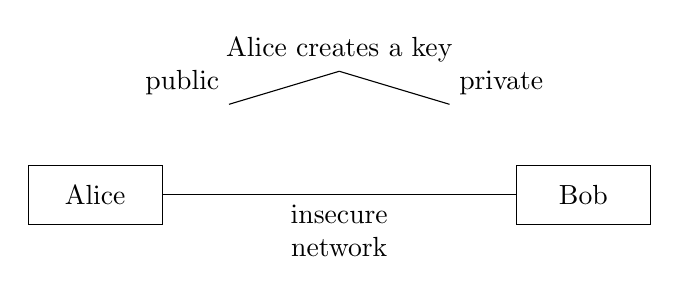
\begin{tikzpicture}[every node/.style={font=\normalsize}]
    \node[draw, minimum width=1.7cm, minimum height=0.75cm] (A) at (0,0) {Alice};
    \node[draw, minimum width=1.7cm, minimum height=0.75cm] (B) at (6.2,0) {Bob};
    \draw (A.east) -- (B.west);
    \node[align=center, below] at (3.1,0) {insecure\\ network};
    \node[align=center] (key) at (3.1,1.85) {Alice creates a key};
    \draw (key.south) -- (1.7,1.15) node[above left] {public};
    \draw (key.south) -- (4.5,1.15) node[above right] {private};
\end{tikzpicture}
\caption{Alice publishes one half of her key. Bob encrypts with the public half; only Alice's private half decrypts. The network between them is insecure.}
\end{figure}

The protocol rests on the difficulty of solving
\[
    x^{e}\equiv C\pmod{N}
\]
for $x$, when $C$, $e$ and $N$ are given.

\paragraph{Step 1: key generation (Alice).}
Alice chooses primes $p$ and $q$, and an encryption exponent $e$. She computes
\[
    N=pq, \qquad \varphi(N)=(p-1)(q-1).
\]

% --- page 35 ---

The exponent $e$ must be coprime to $\varphi(N)$, and the decryption exponent $d$ is its inverse:
\[
    de\equiv 1\pmod{\varphi(N)}.
\]
Alice publishes the public key $(e,N)$ and keeps the private key $(p,q,d)$.

\paragraph{Step 2: encryption (Bob).}
The message is an integer $m$ with $0\le m<N$. Bob computes
\[
    m^{e}\equiv C\pmod{N}
\]
and sends the ciphertext to Alice: $m^{e}\equiv C\pmod{N}$.

\paragraph{Step 3: decryption (Alice).}
Alice computes
\[
    C^{d}\equiv m^{ed}\equiv m\pmod{N},
\]
where the last step is Euler's theorem (or the Chinese remainder theorem, if $\gcdop(m,N)>1$): since $ed=1+\varphi(N)\,t$ for some integer $t$, one has $m^{ed}=m\cdot(m^{\varphi(N)})^{t}\equiv m\pmod{N}$ whenever $\gcdop(m,N)=1$.

\paragraph{When is RSA hard to break?}
The factorization attacks above impose three conditions.
\begin{enumerate}[leftmargin=1.6em]
    \item $p\sim q$, that is, $p$ and $q$ are of about the same size.
    \item $p$ and $q$ should not be too close. (A twin prime is the extreme case: Fermat's search then stops at $N+1^2$.)
    % FIX p.35: ``not'' is inserted with a caret, so that the line reads ``should not be too close'' rather than ``should be too close''.
    \item $p-1$ and $q-1$ should not have very small prime factors. (A Fermat prime is a bad choice: if $p=2^{2^{r}}+1$, then $p-1$ is a power of $2$, and Pollard's $p-1$ method applies.)
\end{enumerate}
% UNCLEAR p.35: a circled mark under item~3 is scribbled out; no fourth condition is readable.

\section{Implementation and Security Issues}
% ============================================================

\subsection{A man-in-the-middle attack}

The attack uses an active adversary on the insecure network, rather than a passive eavesdropper.

\begin{figure}[H]
\centering
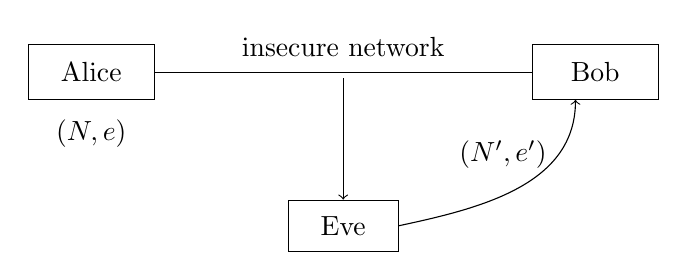
\begin{tikzpicture}
    \node[draw, minimum width=1.6cm, minimum height=0.7cm] (A) at (0,0) {Alice};
    \node[draw, minimum width=1.6cm, minimum height=0.7cm] (B) at (6.4,0) {Bob};
    \draw (A.east) -- (B.west);
    \node[above] at (3.2,0.08) {insecure network};
    \node[anchor=north] at (0,-0.48) {$(N,e)$};
    \node[draw, minimum width=1.4cm, minimum height=0.65cm] (E) at (3.2,-1.95) {Eve};
    \draw[->] (3.2,-0.08) -- (E.north);
    \draw[->] (E.east) to[out=12,in=-90] (6.15,-0.35);
    \node[anchor=west] at (4.55,-1.05) {$(N',e')$};
\end{tikzpicture}
\caption{Eve sits on the channel. She sees Alice's public key $(N,e)$ and substitutes her own key $(N',e')$ on the way to Bob.}
\end{figure}

% --- page 36 ---

Eve has complete control of the insecure network.
\begin{enumerate}[leftmargin=1.6em]
    \item Eve sends Bob a public key $(N',e')$ of her own, in place of Alice's key $(N,e)$. Bob, intending to send a message $m$ to Alice, computes
    \[
        m^{e'}\equiv C'\pmod{N'}
    \]
    and tries to send the ciphertext $C'$ to Alice.
    \item Eve intercepts $C'$. She holds the decryption exponent $d'$ for her own modulus, so
    \[
        (C')^{d'}\equiv (m^{e'})^{d'}\equiv m\pmod{N'}.
    \]
    She then re-encrypts the plaintext under Alice's genuine public key,
    \[
        m^{e}\equiv C\pmod{N},
    \]
    and forwards $C$ to Alice. Alice's decryption recovers the message,
    \[
        C^{d}\equiv m^{ed}\equiv m\pmod{N}.
    \]
\end{enumerate}
Alice receives Bob's message, and at the same time Eve knows it. This is a \emph{man-in-the-middle} attack, also called an \emph{impersonation} attack.

% --- page 37 ---

\subsection{A chosen-ciphertext attack}

\paragraph{Assumption.}
Eve can manipulate Alice.
Listening on the channel, by contrast, is always available to her.

\begin{figure}[H]
\centering
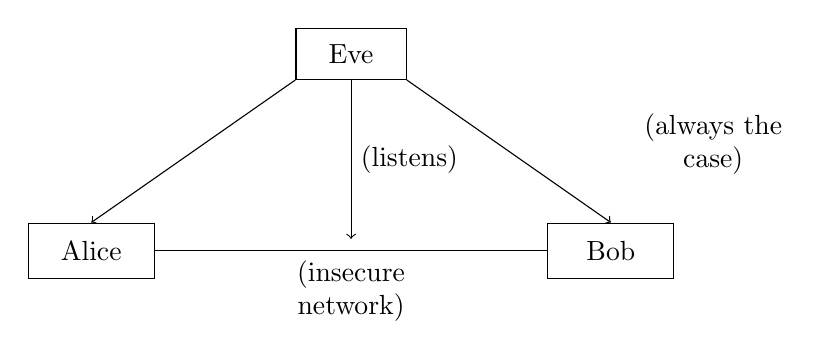
\begin{tikzpicture}
    \node[draw, minimum width=1.4cm, minimum height=0.65cm] (E) at (3.3,2.5) {Eve};
    \node[draw, minimum width=1.6cm, minimum height=0.7cm] (A) at (0,0) {Alice};
    \node[draw, minimum width=1.6cm, minimum height=0.7cm] (B) at (6.6,0) {Bob};
    \draw (A.east) -- (B.west);
    \node[align=center, below] at (3.3,0) {(insecure\\ network)};
    \draw[->] (E.south west) -- (A.north);
    \draw[->] (E.south) -- (3.3,0.15) node[midway, right] {(listens)};
    \draw[->] (E.south east) -- (B.north);
    \node[align=center, anchor=west] at (6.9,1.35) {(always the\\ case)};
\end{tikzpicture}
\caption{Chosen-ciphertext setting. Eve listens on the channel between Alice and Bob (that direction is always open) and can also send messages to Alice.}
\end{figure}

\begin{enumerate}[leftmargin=1.6em]
    \item \textbf{Key generation.}
    Alice's public key is $(N,e)$ and her private key is $(p,q,d)$.
    \item \textbf{Encryption.}
    Let $m$ be the message. Bob sends
    \[
        m^{e}\equiv C\pmod{N}
    \]
    to Alice, and Eve sees $C$. Eve then asks Alice to verify herself, and Alice agrees. Eve chooses an integer $k$ with $1<k<N$ and $\gcdop(k,N)=1$, and sends Alice the altered ciphertext
    \[
        m'\equiv C\,k^{e}\pmod{N}.
    \]
    Alice decrypts and returns
    \[
        S\equiv (m')^{d}\pmod{N}
    \]
    to Eve. Expanding the power,
    \begin{align*}
        (C\,k^{e})^{d}
        &\equiv (m^{e}\,k^{e})^{d}
        \equiv (mk)^{ed}
        \equiv mk \pmod{N}.
    \end{align*}
    So the value Alice sends back is $S\equiv mk\pmod{N}$.
\end{enumerate}
